\documentclass{mprop}
\usepackage{graphicx}
\usepackage{algorithm}
\usepackage{algpseudocode}
\usepackage{float}
\usepackage{siunitx}
\usepackage{xspace}
\usepackage{cite}
\graphicspath{ {images/} }

% alternative font if you prefer
% \usepackage{times}

% for alternative page numbering use the following package
% and see documentation for commands
\usepackage{fancyheadings}


% other potentially useful packages
\usepackage{amssymb,amsmath}
%\usepackage{url}
%\usepackage{fancyvrb}
%\usepackage[final]{pdfpages}

\begin{document}

%%%%%%%%%%%%%%%%%%%%%%%%%%%%%%%%%%%%%%%%%%%%%%%%%%%%%%%%%%%%%%%%%%%
\title{Smooth Latent Dirichlet Allocation in Metabolomics}
\author{Arijus Pleska}
\date{Date of submission placed here}
\maketitle
%%%%%%%%%%%%%%%%%%%%%%%%%%%%%%%%%%%%%%%%%%%%%%%%%%%%%%%%%%%%%%%%%%%

%%%%%%%%%%%%%%%%%%%%%%%%%%%%%%%%%%%%%%%%%%%%%%%%%%%%%%%%%%%%%%%%%%%
\tableofcontents
\newpage
%%%%%%%%%%%%%%%%%%%%%%%%%%%%%%%%%%%%%%%%%%%%%%%%%%%%%%%%%%%%%%%%%%%

%%%%%%%%%%%%%%%%%%%%%%%%%%%%%%%%%%%%%%%%%%%%%%%%%%%%%%%%%%%%%%%%%%%
\section{Introduction}\label{intro}

% Hook intro
\par This research proposal is directed towards applying machine learning in biology. We intend to study the scans of low level biological entities in order to derive their patterns. To be more specific, we aim to tackle the issue of noise, which arises from the hardware limitation of the data collection devices.   

% Metabolomics
\par The branch of biology we are expecting to carry out the research is metabolomics. In brief, metabolomics is the scientific study of chemical processes which involve small molecules -- metamobilites. These chemical processes can be predicted by the features of metabolites; and metabolites are these low level biological entities. By using mass spectrometers, we can obtain the masses and intensities of metabolites. Note that the mass suggests different types of metabolites, whereas the intensity displays the level of concentration. Thereby, a mass spectrum can be used to distinguish and visualise the observed metabolites; and combinations of specific metabolites types   may suggest a specific pattern for the chemical process leading to a particular formation. 

% machine learning in vision
\par In the terms of machine learning applicability, we are looking into a problem of vision. The metabolites of some biological tissue are sequentially captured within regions of fixed size. Effectively, this process is generating an image: each scan is a pixel, therefore, the collections of scans produce an image. However, each pixel contains a large amount of metabolites, so the visualisation of these in a single image would be rather complex. For this reason, we can choose a specific metabolite type and produce pixels reflecting such metabolite activity. Further, we can choose some specific combination (pattern) of metabolites and produce an image of such pattern concentrations. The problem arises upon finding such valid patterns of metabolites, therefore, we are applying machine learning to find the perspective patterns for us. 

% Unsupervised learning > Topic modelling > probabilistic machine learning > LDA > Noise
\par The objective to discover new patterns makes it a problem of unsupervised machine learning. That is, we have no prior settings in how these patterns would look like thus we are utilising machine learning in order to structure the data. The problems of this flavour can be tackled using topic modelling. This branch of unsupervised machine learning is a statistical process. In other words, we are looking into probabilistic models -- the hidden structure of the data is inferred by the frequencies of its instances. To be more specific, we will be focusing on enhancing a particular probabilistic machine learning model -- Latent Dirichlet Allocation (LDA). This model dictates the state-of-the-art of topic modeling and is widely applied in the current research on metabolomics [insert citation]. Since the process of the data collection in metabolomics is prone to noise, we will carry a research on whether Latent Dirichlet Allocation could be applied as a method of error correction. 

\par The structure of this proposal is set-up as follows: in Section 2 we present the issue of noise in Metabolomics; in section 3 we cover the literature in topic modeling which focuses on the variations of Latent Dirichlet Allocation; in Section 4 we provide the metric of success of the proposed research; finally, in Section 5, we go into details on how the project will be executed.

%%%%%%%%%%%%%%%%%%%%%%%%%%%%%%%%%%%%%%%%%%%%%%%%%%%%%%%%%%%%%%%%%%%
\section{Statement of Problem}

% Problem: noise > annotating the data
\par The current mass spectrometry (MS) equipment display a significant accuracy error upon reflecting the exact metabolite construction in a given sample. Rather than relying upon the advances of such equipment, we can investigate the prospect of enhancing the data processing techniques. As described in Section 1, topic modelling is capable to distinguish the hidden structures of metabolites. However, at this point of time, there is no well set generative approach on how to configure Latent Dirichlet Allocation to reduce the impact of noise in a given dataset.  

% Objectives: utilise LDA to correct the errors
\par The primary goal of this research is to expand the consensus on whether topic modelling is a valid of approach to smooth datasets. To be more specific, the objectives we will be looking into are listed as follows:
\begin{enumerate}
    \item Adapt and utilise the generative Latent Dirichlet Allocation models in metabolomics;
    \item Reduce the impact of noise in the datasets of metabolomics;
    \item Give a basis to the generative Latent Dirichlet Allocation model in error correction.
\end{enumerate}
The first objective is expected to investigate the perspective applications of topic modelling which are successfully utilised in other domains. Effectively, we want to assess the general models (or models displaying significant results in other fields). The second objective would adapt, and thus enhance, these general models for the particular use of error correction in metabolomics. Finally, the third objective can be treated as a general contribution to the field of machine learning. 

% Hypothesis: topic modelling can be utilised in the error correction
\par We are setting a hypothesis that topic modelling, or more specifically Latent Dirichlet Allocation, can be utilised to correct the errors in the datasets of metabolomics. Both cases of proving and disproving this hypothesis would be a contribution in metabolomics. The successful outcome would lead to the potential applications provided in the following paragraph, whereas the unsuccessful outcome would set-up additional requirements to tackle this issue.

% Results: tools to annotate the metabolites > basis for generative error correction 
\par The potential applications of this research can be induced directly induced from the set-up objectives. First of all, we would show that models from other domains can be applied in metabolomics and, thus, generalised. Further, the developed error correction methodology for the datasets of Metabolomics would improve the accuracy of the chemical processes prediction. Finally, the generalisation of the developed error correction methodologies would provide an alternative tool-kit for other domains as well as expand the potential applications of the results derived from metabolomics. 


%%%%%%%%%%%%%%%%%%%%%%%%%%%%%%%%%%%%%%%%%%%%%%%%%%%%%%%%%%%%%%%%%%%
\section{Background Survey}

% intro
\par The provided literature review on latent Dirichlet allocation assesses its underlying methodology and proposes several different implementation variations. The review is structured in progressing order: to start with, we look into the original latent Dirichlet allocation paper and define the terminology which will be used throughout this proposal; then, we familiarise with two different approaches used for the inference of latent Dirichlet allocation;  finally, we review the perspective advances which could be used for error correction.

\subsection{Terminology}

% Topic modelling in a nutshell > Example
\par Recall that in topic modelling we are trying to induce some hidden structure within the studied data. For instance, if we were analysing a book, it would be likely to address several different topics. Further, the chapters of the book itself would have unique concentrations of such topics. In order to cluster these topics, a probabilistic topic modelling method would look into the structure of the words used in the book. Also, the performance of the method would depend on its ability to optimise this clustering, for example, we could dismiss the commonly used words such as: and, or, the, etcetera. Note that in we will assess only the topic modelling where we do not know the naming of topics. That is, we will be looking into a \textit{unsupervised learning} problem.

% Terminology
\par The terminology used in this proposal is equivalent to the one used in the survey on probabilistic topic models carried by Blei et al. [citation]. Figure \ref{fig:lda} below represents the latent Dirichlet allocation model in plate notation. We will use it as a guide to familiarise with the terminology.   
\begin{figure}[H]
  \centering
  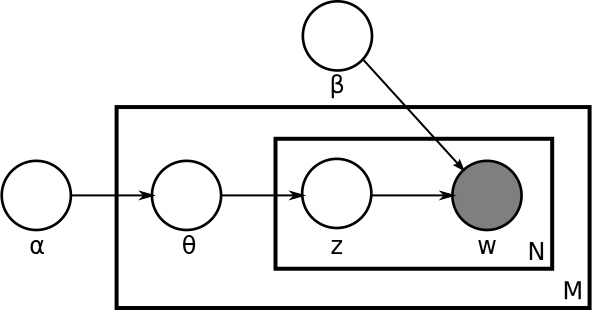
\includegraphics[width=0.7\textwidth]{lda}
  \caption{Latent Dirichlet allocation. COPYRIGHT. CHANGE M TO D}
  \label{fig:lda}
\end{figure}

% High level terminology.
\par To start with, we will familiarise with the domain of the model in a high level. The grey circle represents a single word, whereas a collection of words (document) is represented by the inner plate, and the outer plate corresponds to a collection of documents (corpus). In the model, words are the only \textit{observable variables} -- this is indicated by the grey colour of the circle, whereas the white coloured circles indicate the \textit{hidden variables}. As suggested by the figure, a \textit{word} is denoted by $w$; a \textit{document} (sequence of words) is denoted by $\mathbf{w} = \{w_1, w_2, \dots, w_N\}$, where $N$ indicates the number of words in the document; and a \textit{corpus} is denoted by $\mathcal{\mathbf{D}} = \{\mathbf{w_1}, \mathbf{w_2}, \dots, \mathbf{w_M}\}$, where $D$ is the number of documents in the corpus. 
 
% Low Level terminology.
\par Now, we will introduce the lower level entities -- the hidden variables. Recall that latent Dirichlet allocation attempts to induce an arbitrary mixture of topics. The corpus and each document is expected to vary in the proportions of the induced topics; and each document is likely to have a different number of word. Let's denote the number of such arbitrary topics by $K$, and the number of unique words in the corpus by $V$. This notation will simplify the explanation on the remaining entities in Figure \ref{fig:lda}. To start with, $\beta$ is the hyper-parameter (a matrix of dimension $V \times K$) referring to the prior distribution of the topics over the vocabulary. The hyper-parameter $\alpha$ (a vector of length $K$) refers to the prior distribution of the topics over the documents. Further, the latent variable $\theta$ (a matrix of dimension $D \times K$) is the topic distribution over documents. Finally, $z$ is the latent variable on the topic assignments of each word in every document, effectively, it is a matrix of dimension $M \times V$.

\subsection{Preliminaries}
% Relationship between the variables.
% To-do: COPYRIGHT for the equation.
\par The relationship between observable and hidden variables, effectively, describes the inference of the underlying topic structure. We will go through an arbitrary example in order to give intuition in the inference process and provide the notation of the variable instances. By looking into Figure \ref{fig:lda}, we can see that $\alpha_k$ (the prior weight of the $k$th topic in a document) influences $\theta_{:, k}$ (the latent $k$th topic distribution over $M$ documents). It follows that $\theta_{d, k}$ (the probability of the $k$th topic occurrence in the document $d$) influences $z_{d, :}$ (the topic assignment over $V$ vocabulary terms in document $d$). Note that $z_{d, v}$ would refer to the assignment of some specific vocabulary term $v$. Now, by taking $z_{d, v}$ and $\beta_{v, k}$ (the prior weight of the $k$th topic on the vocabulary $v$) we describe the origins of word $w_{d, v}$. The relationship of the terms, effectively, induces the generation of the corpus, this can be expressed as the following joint probability distribution
\begin{equation}
p(\beta, \theta, z, w) = \prod_{k=1}^Kp(\beta_{:, k})\prod_{d=1}^Dp(\theta_{d, :})\bigg(\prod_{v=1}^Vp(z_{d, v} | \theta_{d, :})p(w_{d, v} | \beta, z_{d, v})\bigg).
\end{equation}
By using Bayes Theorem, we derive the computation of the conditional distribution
\begin{equation}
p(\beta, \theta, z | w) = \frac{p(\beta, \theta, z, w)}{p(w)}. 
\end{equation}
This equation expresses the computation of the posterior -- the derivation of the hidden corpus structure given observable variable $w$. The problem arises from inefficient analytical computation of evidence $p(w)$. By reviewing the literature on latent Dirichlet allocation [CITATION], we will also familiarise with the numerical methods used in approximating $p(w)$.

% Intro > methodology > experiments
\subsection{Latent Dirichlet allocation}

% Intro:
% Attention to detail giving a basis fo the following model interpretations
\par Latent Dirichlet allocation is a probabilistic topic modelling technique  proposed by Blei et al [citation]. Since this subsection is dedicated for the origins of the technique, it will be broader in detail. This will cover aspects addressed in the following subsections covering the advances on latent Dirichlet Allocation. 

% Assumptions: 
% - Exchengable docs and words > bag of words
% - Discrete data
% - Dimensionality of topic variable is assumed to be known and fixed\
\par The initial latent Dirichlet allocation model sets some assumptions for the data which will be processed by the model. First of all, it is assumed that both documents and words in the documents are \textit{exchangeable}. That is, the order in which these will be processed does not matter. More formally, this assumption means that the model follows the \textit{bag-of-words} principle. The next assumption is that the model works on discrete data. Effectively, the original paper does not cover the treatment of continuous features. Another assumption is on the dimensionality of the topic variables: the number of topics is set to be fixed during the complete run of inference.  

% Document Generation:
% - Algorithm
% - Alpha and Beta are sampled once, whereas w and z are sampled once per each word in a document
% - Three level bayesian hierarchy~~
\par As discussed in the preliminaries subsection, the process of latent Dirichlet allocation assumes that the corpus can be generated by a probabilistic process. The generation of the corpus is made of three levels: the parameters $\alpha$ and $\beta$ are sampled once; the variable $\theta$ is sampled once per document; and the variables $z$ and $w$ are sampled once per word. The generative algorithm given in the original paper is equivalent to Algorithm 1 below.
\begin{algorithm}[H]
\caption{Document Generation.}
\label{alg:document_generation}
\begin{algorithmic}[1]
% \Procedure {generate_document}{$\xi, \alpha, \beta$}
\State $N \sim \mbox{Poisson}(\xi)$
\State $\theta \sim \mbox{Dir}(\alpha)$
\For {$n \leftarrow 1, N$}
\State $z_n \sim \mbox{Multinomial}(\theta)$
\State $w_n \sim \mbox{p}(w_n | z_n, \beta)$
\EndFor
% \EndProcedure
\end{algorithmic}
\end{algorithm}
Note that the algorithm describes the generation of a single document. In order to generate the corpus, we would run the algorithm several times. To start with, in the line 1 we draw the number of words in the document $N$, where $\xi$ is an ancillary variable suggesting the mean for the Poisson Distribution. In the line 2 we draw the topic distribution $\theta$ from the Dirichlet distribution on $\alpha$. Now in the lines 3--6 we generate the words: in the line 4 we draw topic $z_n$ from the multinomial distribution on $\theta$; and, finally, in the line 5 we obtain the word $w_n$ from the conditional probability on $z_n$ and the distribution over the words in the vocabulary $\beta$.


% Inference
% - Setting alpha and beta as hypterparameters, i.e. reforming the posterior formula. (untouched)
% - Variational inference: variational parameters gamma and fi
\par The inference is, effectively, the computation of the evidence for the posterior distribution. The original latent Dirichlet allocation paper uses the method of variational inference. Basically, the authors introduce the variational parameters $\gamma$ and $\phi$ (computation of these set-ups a problem of optimisation). Note that the original paper provides pseudo code for solving the optimisation problem.

% Parmeter estimation
% - M Step update for beta
% - Update for alpha using newton-raphson method
% Problem with smoothing: Large datasets > sparsity, training corpus blocks the possibility of the new words coming from new documents
\par Additionally, the authors emphasise the estimations of the parameters $\alpha$ and $\beta$. They suggest a two-step EM procedure utilising the variational parameters $\gamma$ and $\phi$: E-step is the optimisation problem addressed in the previous paragraph; and M-step updates the parameters $\alpha$ and $\beta$. Note that the authors provide an analytical update for $\beta$ and a Newton--Raphson method for updating $\alpha$. Apart from that, the authors also introduce the issue of a sparse corpus. Such corpus would be expected upon having a large vocabulary or a significant amount of documents. The authors suggest addressing this problem by introducing smoothing. They introduce an additional parameter $\eta$ which impacts the estimation of $\beta$. 

% Experiments:
% - Document modelling: issue with pLSI and mixture unigrams~; perplexity (UNTOUCHED)
% - Document classification: dimensionality reduction; comparison with SVM
\par The conducted experiments display the improvement performance over the predecessor models and suggest the application domain of latent Dirichlet allocation. The first experiment addresses document modelling. The latent Dirichlet allocation model is reported to display balanced hidden topic proportions in the set of test documents. That is, the test set has replicated the proportions of the training set. The second experiment addresses document classification. In order to display better performance compared to a support vector machine (SVM) model, the authors address the dimensionality reduction of the tested documents. This means that the documents would possess a lower amount of features. It follows that the latent Dirichlet allocation model has successfully reduced the number of features and displayed an improvement in accuracy compared to the support vector machine model. 

% Discussion and Conclusion
\par The review on the initial latent Dirichlet allocation model has set-up a basis for introducing the successor variations. These will be provided in the following sections. We have introduced the initial methodology for the following reasons: (1) the novel models will display the relaxation of the initial assumptions; (2) the provided document generation methodology will be compared to the document generation in batches; (3) we will cover different inference and parameter estimation approaches. Also, note that the paper is relatively old in time, and the experiments do not display the state-of-the-art performance. Rather than that, they were introduced to address the application domains of the model. 

\subsection{Dynamic Topic Models}

% Intro:
% - Time series
% - Both qualitative and quantitative results
\par Now we review the paper on Dynamic Topic Models [CITATION]. Effectively, the dynamic topic model can be treated as an extension of static topic models (such as latent Dirichlet allocation). The main idea behind a dynamic topic model is that it induces the topic evolution the processed corpus. That is, the documents in the corpus evolve over time. In this subsection, we review the key assumptions of dynamic topic models, go over the generative process of documents, review the suggested inference methods, and familiarise with the results of the carried experiment. 

% Assumptions:
% - Data is divided in time slices
\par We will emphasise the assumptions given on the dynamic topic models. First of all, even though we are discussing a model of time series suggesting the use of continuous variables, the data remains categorical. The distinction between continuous and categorical data is that continuous data is strictly numeric and infinite, whereas categorical data can take only particular values. The second assumption relaxes the ex-changeability on documents. That is, the documents are expected to form a sequence. Or in other words, the corpus is divided into time-slices. Note that in such time-slice documents are exchangeable.  

% Generative Process:
\par The generative process of the models updates the parameters $\alpha$ and $\beta$. This means that the topic distributions over documents and words change over time. The visualisation of the process is given in Figure 2 below.
\begin{figure}[H]
  \centering
  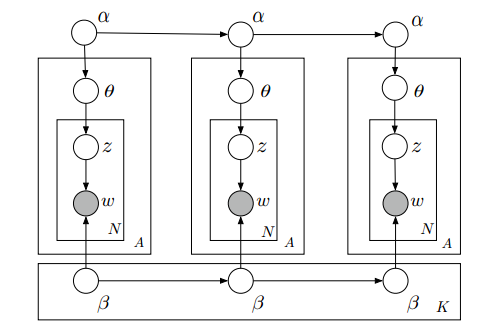
\includegraphics[width=0.7\textwidth]{dynamic_topic_model}
  \caption{Dynamic topic model. COPYRIGHT.}
  \label{fig:dtm}
\end{figure}
Notice that each time-slice is equivalent to the model shown in Figure 1. Also, the parameters $\alpha$ and $\beta$ are induced by their predecessors in the previous time-slice. More formal representation of the generative process is given in Algorithm 2. 
\begin{algorithm}[H]
\caption{Dynamic document generation.}
\label{alg:dynamic_document_generation}
\begin{algorithmic}[2]
\State $\beta_t | \beta_{t-1} \sim \mathcal{N}(\beta_{t-1}, \sigma^2)$
\State $\alpha_t | \alpha_{t-1} \sim \mathcal{N}(\alpha_{t-1}, \delta^2)$
\For {$d \leftarrow 1, D$}
\State $\eta_d \sim \mathcal{N}(\alpha_{t}, a^2)$
\For {$n \leftarrow 1, N$}
\State $z_{d, n} \sim \mbox{Multinomial}(\pi(\eta_d))$
\State $w_{t, d, n} \sim \mbox{Multinomial}(\pi(\beta_t | z_{d, n}))$
\EndFor
\EndFor
% \EndProcedure
\end{algorithmic}
\end{algorithm}
The given algorithm describes the generative process for the time-scale $t$. It starts by drawing the parameters $\alpha_t$ and $\beta_t$ from the Gaussian distribution with the means given by the previous parameter values. For now, we will not discuss the meaning of the variance values. Further, for each document in the time-scale, we carry the following procedure: we draw the topic distribution in a document $\eta_d$ from the Gaussian distribution with the mean given by $\alpha_t$; then, for each word in the document, we draw the topic $z_{d, n}$ from the Multinomial distribution on the parametrised $\eta_d$, and, finally, we draw the word $w_{t, d, n}$ from the Multinomial distribution on the parametrised $\beta_t$ which is conditioned on $z_{d, n}$. By the use of \textit{parametrisation}, we are expressing the result of the Gaussian distributions into a format suitable for Multinomial distribution. This mapping is expressed as
\begin{equation}
\pi(x)_n = \dfrac{\exp{(x_n)}}{\sum^n_{i=1}\exp{(x_i)}}.
\end{equation}

% Inference:
% Variational methods are a deterministic alternavive for stochastic simulation
% Two variations: Kalman filter and wavelet regression
\par The authors suggest using variational methods to approximate the inference posterior. It is claimed that stochastic simulation would be unable to scale with large data sets. Two techniques of variational methods are provided: Kalman Filtering and Wavelet Regression. The implementation details of these are provided in a brief manner suggesting the computation of the parameter $\beta_t$. 

% Experiments:
% - Evolution of Science
\par The dynamic topic model is evaluated by conducting an experiment on the journals of \textit{Science}. The experiment is expected to establish the time series on the topic development with the articles. Indeed, the experiment is able to produce results displaying the rises and falls of the topics indicating scientific fields. Note that the experiment is performed using both variational inference methods.   

% Concluison
\par The review on the dynamic topic models has familiarised us with more realistic generative process: the documents are induced by time series. Further, we have provided the visualisation of the model and introduced the algorithm for the generative process. Also, we have captured the techniques used for inference. Finally, we have familiarised with the experiment settings. 






%%%%%%%%%%%%%%%%%%%%%%%%%%%%%%%%%%%%%%%%%%%%%%%%%%%%%%%%%%%%%%%%%%%
\section{Proposed Approach}

state how you propose to solve the software development problem. Show that your proposed approach is feasible, but identify any risks.

%%%%%%%%%%%%%%%%%%%%%%%%%%%%%%%%%%%%%%%%%%%%%%%%%%%%%%%%%%%%%%%%%%%
\section{Work Plan}

show how you plan to organize your work, identifying intermediate deliverables and dates.

%%%%%%%%%%%%%%%%%%%%%%%%%%%%%%%%%%%%%%%%%%%%%%%%%%%%%%%%%%%%%%%%%%%
% it is fine to change the bibliography style if you want
\bibliographystyle{plain}
\bibliography{mprop}
\end{document}


% To-do: relaxing the matrix dimension assumptions, i.e., introducing the dictionary variation